% !TEX root = ../main.tex

\section*{Control system}

In order to control the launch remotely, a simple electronic system has been build. This system is connected to different power sources and to a data-logger that connects to a computer acting as a server.

\subsection*{Software}

\begin{figure}[H]
  \centering
  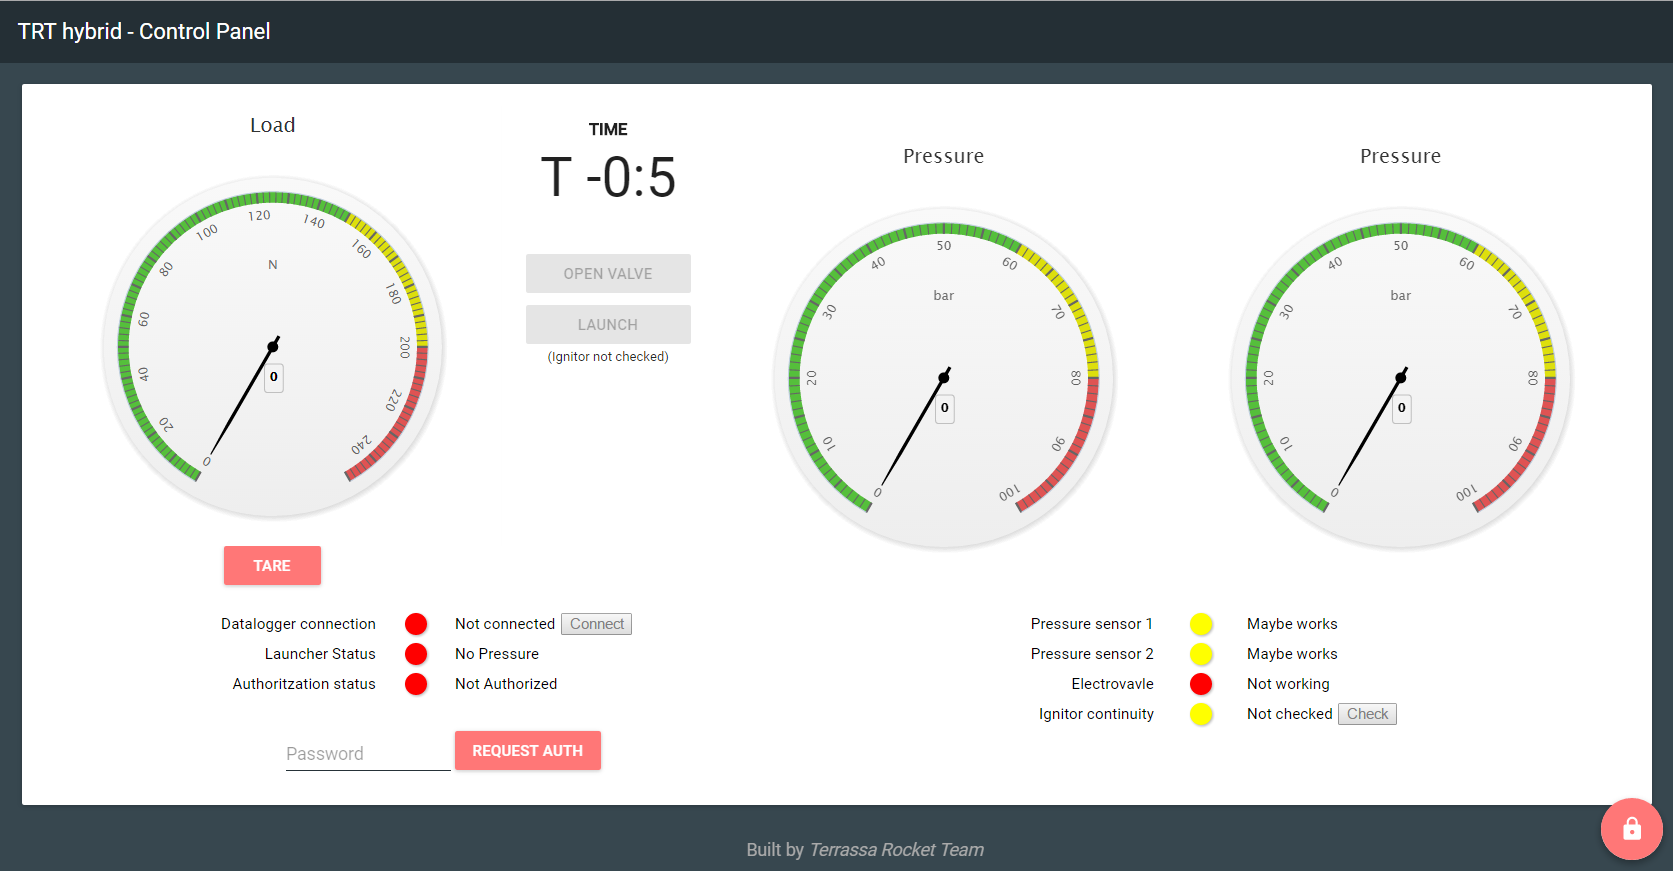
\includegraphics[width=0.8\textwidth]{controlPanel.png}
  \caption{Software screenshot}
  \label{fig:softwareScreenshot}
\end{figure}

After the server is initialized, clients can connect to it using a standard web-browser from any device. Any client is able to see the data from the sensors and, after proper authentication, they are able to control the gas valve and, the continuity check of the ignitor and the ignitor trigger. The data is always stored in the server at the full sampling rate, but the clients only receive the mean of the last 0.1 seconds.

The server is implemented using javascript and node.js. The server connects to the serial port using the "serialport" package and uses "websockets" to send the sensors data in real time to the clients. The interface between the data-logger and the server has been specially developed for this program based on previous experience writing an open-source library for Matlab for the same data-logger.

The clients web pages are implemented in React and Redux from Facebook. The charts use the library "highcharts".

The full implementation of the code can be found on \cite{hybridControlPanelGithub}. A screenshot of the clients software can be seen on Figure \ref{fig:softwareScreenshot}.

\subsection*{Electronics}

\begin{figure}[H]
  \centering
  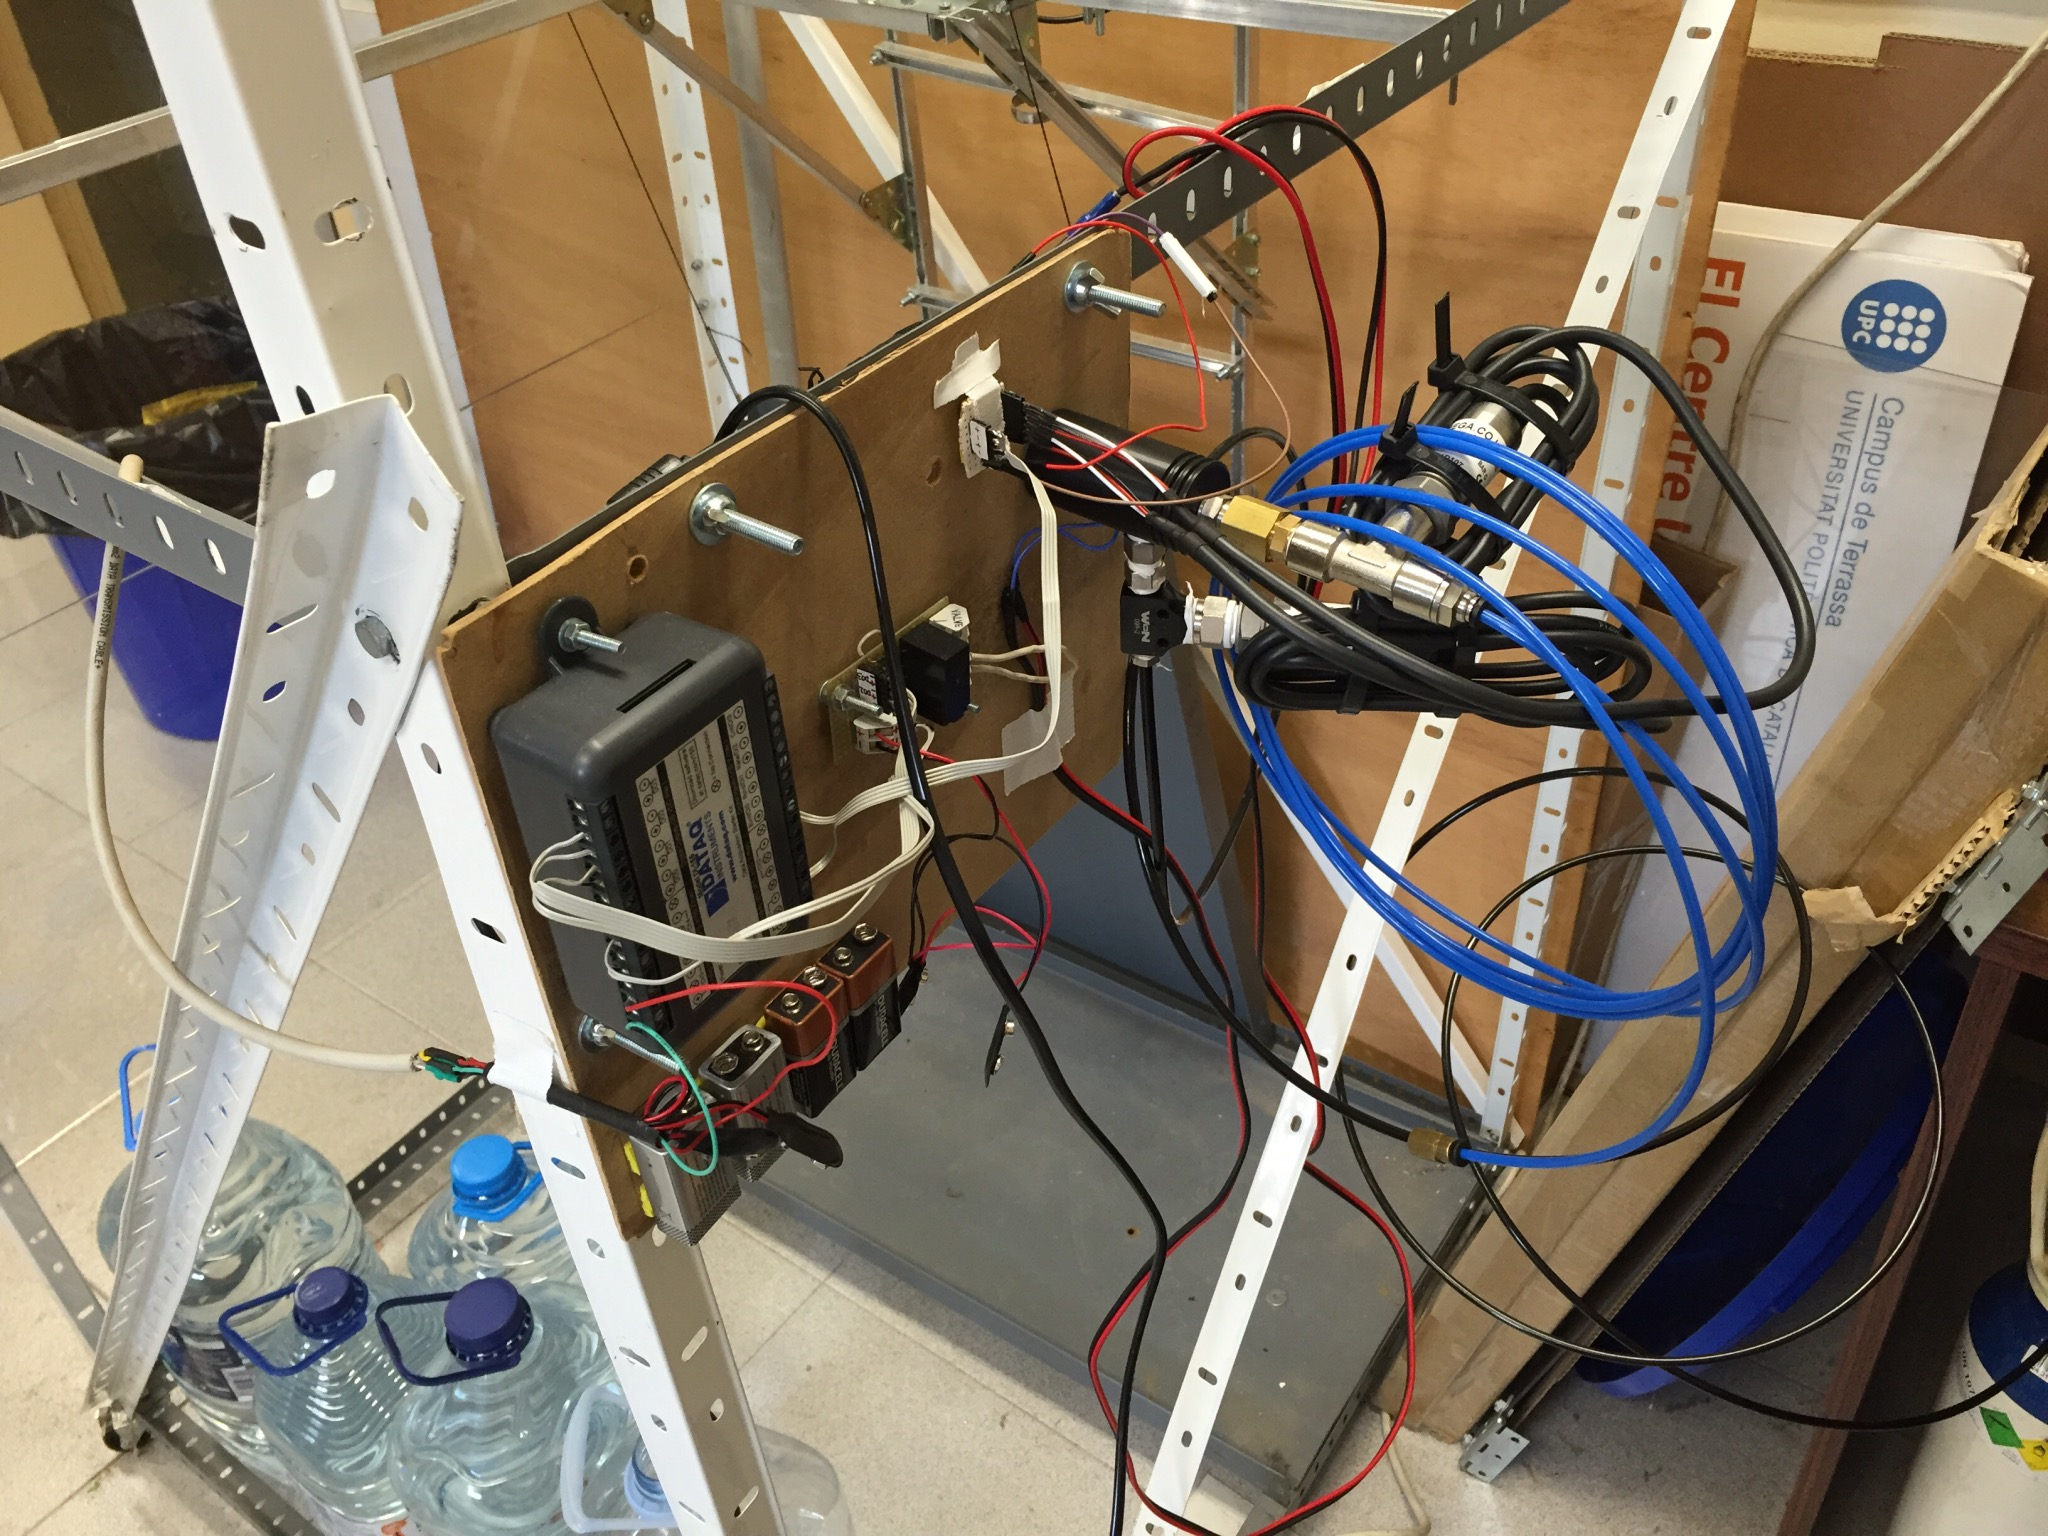
\includegraphics[width=0.8\textwidth]{electronica.jpg}
  \caption{Electronics}
  \label{fig:electronica}
\end{figure}

The electronics to connect the sensors and actuators with the DI-155 data-logger from DataQ are also custom for this case.

There are 4 sensors attached to the fire test machine:
\begin{itemize}
  \item 2 pressure transductors provided by Omega.
  \item 1 load cell for measuring up to 50Kg of force.
  \item 1 continuity check for the ignitor
\end{itemize}

And 3 actuators:
\begin{itemize}
  \item 1 ignitor check trigger
  \item 1 ignitor fire trigger
  \item 1 gas electrovavle trigger
\end{itemize}

An image of the electronics can be seen on the previous Figure \ref{fig:electronica}.
